\chapter{Variables and arithmetic}

This chapter is about storing values in computer memory and doing basic arithmetic.
More importantly, it discusses how to {\em compose} statements using smaller building blocks such as variables, literals, and operators.
We also discuss code quality, which is almost as important as correctness.
High quality code is easier to read, which makes it easier to debug.


\section{Types of errors}

\index{error!message}

Three kinds of errors can occur in a program: syntax errors, runtime errors, and logic errors.
It is useful to distinguish between them in order to track them down more quickly.
Regardless of what type of error occurs, remember to {\em read and think about the error messages carefully}.
They will usually point you in the right direction to fix your program.

\subsection{Syntax errors}

\index{syntax error}
\index{error!syntax}

The compiler can only translate a program if the syntax is correct; otherwise, it fails and displays an error message.
For example, parentheses have to come in matching pairs.
So \java{(1 + 2)} is legal, but \java{8)} is a {\bf syntax error}.

In English, readers can tolerate most syntax errors, which is why we can read the poetry of E.\ E.\ Cummings without spewing error messages.
Java is not so forgiving; if there is a single syntax error anywhere in your program, the compiler will display an error message and quit, and you will not be able to run the program.

\begin{figure}[!h]
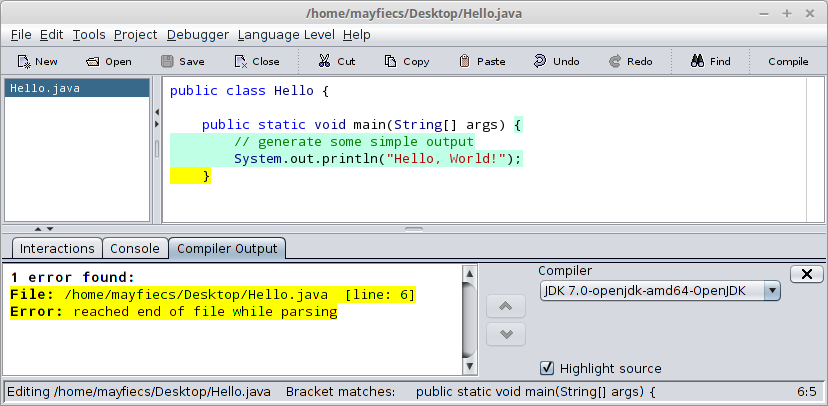
\includegraphics[width=\textwidth]{syntax-error.png}
\caption{A syntax error caused by a missing brace.}
\end{figure}

% ABD: This figure should have a number, and we should refer to it in the
% text.

To make matters worse, the error messages you get from the compiler are often not very helpful.
For example, removing the closing brace on line 8 of the hello world program results in ``Error: reached end of file while parsing.''
The compiler also reports that the problem was found on line 6, which in this case is not at fault.

During the first few weeks of your programming career, you will probably spend a lot of time tracking down syntax errors.
But as you gain experience, you will make fewer mistakes and find them more quickly.

\subsection{Runtime errors}

\index{runtime error}
\index{error!runtime}
%\index{type-safe}
%\index{language!type-safe}

The second type of error is a runtime error, so called because it does not appear until after the program has started running.
In Java, these errors occur when the interpreter is executing the byte code and something goes wrong.
%Java is designed to be a {\bf type-safe} language, which means that the compiler can detect many potential errors cased by common programming mistakes.
Runtime errors are rare in the simple programs you will see in the first few chapters, so it might be a while before you encounter one.

\index{exception}

These errors are also called {\bf exceptions} because they usually indicate that something exceptional (and bad) has happened.
In most environments they appear as windows or dialog boxes that contain information about what happened and what the program was doing when it happened.
For example, if you accidentally divide by zero you will get an \java{ArithmeticException}:

\begin{small}
\begin{stdout}
Exception in thread "main" java.lang.ArithmeticException: / by zero
    at Hello.main(Hello.java:5)
\end{stdout}
\end{small}

This information is useful for debugging.
The first line gives a brief description of the error (/ by zero).
The subsequent lines report the class and method names (Hello.main), along with the file name and line number where the error occurred (Hello.java:5).
Keep in mind that the line where the program crashed may not be the line that needs to be fixed.

\subsection{Logic errors}

\index{logic error}
\index{error!logic}

The third type of error is the {\bf logic error}.
If there is an error in your program's logic, it will compile and run successfully in the sense that the computer will not generate any error messages.
But it will not do the right thing.
It will do something else.
Specifically, it will do what you told it to do.
Here is an example of a logic error in the hello world program:

\begin{code}
public class Hello {

    public static void main(String[] args) {
        System.out.println("Goodbye, world.");
    }

}
\end{code}

This program compiles and runs just fine.
The problem is that the main method is not the program we intended.
The meaning of the program is wrong, because it says goodbye instead of hello.
In addition, world is not capitalized, and it ends with a period instead of an exclamation point.

Identifying logic errors can be tricky because it requires you to challenge your assumptions, both about the code and the requirements.
You will need to work backwards by looking at the output of the program, try to figure out what it is doing, and make sure you understand what it should be doing.


\section{Creating variables}

\index{variable}
\index{value}

One of the most powerful features of a programming language is the ability to define and manipulate {\bf variables}.
A variable is a named location of computer memory that stores a {\bf value}.
Values may be numbers, text, images, sounds, and other types of data.
%They can be printed, and as we'll see later, operated on.
To store a value in memory, you first have to create a variable.
%Since the values we want to store are text, we declare that the new variable is a string:

\begin{code}
    String message;
\end{code}

\index{declaration}
\index{statement!declaration}
\index{type!int}
\index{type!char}
\index{type!String}

This statement is a {\bf declaration}, because it declares that the variable named \java{message} has the type \java{String}.
Each variable has a {\bf type} that determines what kind of values it can store.
For example, the \java{int} type can store integers, and the \java{char} type can store characters.

Some types begin with a capital letter and some with lower-case.
We will learn the significance of this distinction later, but for now you should take care to get it right.
There is no such type as \java{Int} or \java{string}, and the compiler will complain if you make one up.

To declare an integer variable, the syntax is:

\begin{code}
    int x;
\end{code}

Note that \java{x} is an arbitrary name for the variable.
In general, you should use names that indicate what the variables mean.
For example, if you saw these variable declarations, you could probably guess what values would be stored in them:

\begin{code}
    String firstName;
    String lastName;
    int hour, minute;
\end{code}

This example also demonstrates the syntax for declaring multiple variables with the same type: \java{hour} and \java{second} are both integers.
Note that each declaration statement ends with a semicolon.

You can use any name you want for a variable or constant.
But there are certain words that are reserved in Java, because they are used by the compiler to parse the structure of the program.
The {\bf keywords} include \java{public}, \java{class}, \java{static}, \java{void}, \java{int}, and others (there are currently 50 in Java).
Search the Internet for ``Java keywords'' to see the complete list.

%The complete list is available at \url{https://docs.oracle.com/javase/tutorial/}.
%This site, provided by Oracle, includes Java documentation I refer to throughout the book.

Rather than memorize the keywords, you should take advantage of the syntax highlighting provided in many development environments (including DrJava).
As you type, the tokens in your program will appear in different colors.
For example, keywords might be blue, strings red, comments green, and other code black.
If you type a variable name and it turns blue, watch out!


\subsection{Assignment}

\index{assignment}
\index{statement!assignment}

Now that we have created variables, we want to store values.
We do that with an {\bf assignment} statement.

\begin{code}
    message = "Hello!";  // give message the value "Hello!"
    hour = 10;           // assign the value 10 to hour
    minute = 59;         // set minute to 59
    hour = 11;           // change the hour to 11
\end{code}

This example shows four assignments, and the comments illustrate different ways people sometimes talk about assignment statements.
The vocabulary can be confusing here, but the idea is straightforward:

\begin{itemize}
\item When you declare a variable, you create a named storage location.
\item When you make an assignment to a variable, you give it a value.
\item If you reassign the variable, its value changes.
%The storage location does not change; those memory cells are simply reused.
\end{itemize}

As a general rule, a variable has to have the same type as the value you assign to it.
For example, you cannot store a \java{String} in \java{minute} or an integer in \java{message}.
We will see some examples that seem to break this rule, but we'll
get to that later.

%On the other hand, that rule can be confusing.
%There are many ways that you can convert values from one type to another, and Java sometimes converts things automatically.
%For now you should remember the general rule, and we'll talk about exceptions later.

A common source of confusion is that some strings {\em look} like integers, but they are not.
For example, \java{message} can contain the string \java{"123"}, which is made up of the characters \java{'1'}, \java{'2'}, and \java{'3'}.
But that is not the same thing as the integer \java{123}.

\begin{code}
    message = "123";  // legal
    message = 123;    // not legal
\end{code}


\subsection{Memory diagrams}

\index{memory diagram}

A common way to represent variables on paper is to draw a box with the name of the variable on the outside and the value of the variable on the inside.
This diagram shows the effect of the four assignments in the previous section:

\begin{center}
\begin{tabular}{rl}
message & \framebox[2cm]{Hello!} \\
   hour & \framebox[1cm]{11} \\
 minute & \framebox[1cm]{59} \\
\end{tabular}
\end{center}

% ABD: In the hour box, consider showing 10 crossed out, followed by 11?

Each box represents the storage location that holds the variable's value.
%Since these locations can be anywhere in memory, we refer to them by the variable name.
Once declared, you cannot change the name of a variable, but you can change the value as many times as you like.  For example, \java{hour} was
initially 10, then reassigned to 11.  The diagram shows only the final
value.


\section{Printing variables}
\label{sec:printvar}

You can display the value of a variable using \java{print} or \java{println}.
The following program declares a variable named \java{firstLine}, assigns it the value \java{"Hello, again!"}, and then prints that value.

\begin{code}
public class Hello {
    public static void main(String[] args) {
        String firstLine;
        firstLine = "Hello, again!";
        System.out.println(firstLine);
    }
}
\end{code}

When we talk about printing a variable, we generally mean printing the {\em value} of the variable.
To print the {\em name} of a variable, you have to put it in quotes.
%For example: {\tt System.out.println("firstLine");}
For example, you can write:

\begin{code}
    String firstLine;
    firstLine = "Hello, again!";
    System.out.print("The value of firstLine is ");
    System.out.println(firstLine);
\end{code}

The output of this program is:

\begin{stdout}
The value of firstLine is Hello, again!
\end{stdout}

The output does not contain quote marks around \java{Hello, again!}.
Those quote marks were part of the source code, not the value.

The syntax for printing a variable is the same regardless of the variable's type.
For example:

\begin{code}
    int hour, minute;
    hour = 11;
    minute = 59;
    System.out.print("The current time is ");
    System.out.print(hour);
    System.out.print(":");
    System.out.print(minute);
    System.out.println(".");
\end{code}

The output of this program is:

\begin{stdout}
The current time is 11:59.
\end{stdout}

To output multiple values on the same line, it's common to use several \java{print} statements followed by a \java{println} at the end.
{\bf Don't forget the {\tt println}!}
On many operating systems, the output from \java{print} is stored without being displayed until \java{println} is invoked, at which point the entire line is displayed at once.
If you omit the {\tt println}, the program may display the stored output at unexpected times or even terminate without displaying anything.


% ABD: I'd like to postpone the discussion of final variables.  At
% this point I think they solve a problem the students don't understand
% yet.



\section{Arithmetic operators}

\index{operator}
{\bf Operators} are symbols that represent computations like addition and multiplication.
For example, the operator for addition is \java{+}, subtraction is \java{-}, multiplication is \java{*}, and division is \java{/}.

The following program converts the time of day to minutes:

\begin{code}
    int hour, minute;
    hour = 11;
    minute = 59;
    System.out.print("Number of minutes since midnight: ");
    System.out.println(hour * 60 + minute);
\end{code}

In this program, \java{hour * 60 + minute} is an {\bf expression},
which is a combination of numbers, variables, and operators.
The the program runs, each variable is replaced by its value, and
then the operators are applied to the values.

The result is:

\begin{stdout}
Number of minutes since midnight: 719
\end{stdout}

Addition, subtraction, and multiplication all do what you expect, but you might be surprised by division.
For example, the following lines try to compute the fraction of
an hour that has elapsed:

\begin{code}
    System.out.print("Fraction of the hour that has passed: ");
    System.out.println(minute / 60);
\end{code}

Bu the program outputs:

\begin{stdout}
Fraction of the hour that has passed: 0
\end{stdout}

\index{division!integer}
\index{integer division}
\index{operand}

This result often confuses people.
After all, the value of {\tt minute} is 59, and 59 divided by 60 should be 0.98333, not 0.
The problem here is that Java is performing {\em integer division}.
When the values being divided are integers, the result is also an integer.
Computer hardware is designed so that integer division always rounds {\em down}, even in cases like this one where the next integer is close.

One solution is to calculate a percentage rather than a fraction:

\begin{code}
    System.out.print("Percent of the hour that has passed: ");
    System.out.println(minute * 100 / 60);
\end{code}

The new output is:

\begin{stdout}
Percent of the hour that has passed: 98
\end{stdout}

Again the result is rounded down, but at least now it's approximately correct.


\section{Floating-point numbers}

\index{floating-point}
\index{double (floating-point)}
\index{type!double}

A more general solution is to use {\bf floating-point} numbers, which can represent fractions as well as integers.

In Java, the default floating-point type is called \java{double}, which is short for double-precision.
You can create \java{double} variables and assign values to them using the same syntax we used for the other types:

\begin{code}
    double pi = 3.14159;
\end{code}

Although floating-point numbers are useful, they 
can be a source of confusion.
For example, Java distinguishes the integer value {\tt 1} from the
floating-point value {\tt 1.0}, even though they seem to be the same
number.  They belong to different data types, and strictly speaking,
you are not allowed to make assignments between types.

The following is illegal because the variable on the left is an \java{int} and the value on the right is a \java{double}.

\begin{code}
    int x = 1.1;  // syntax error
\end{code}

But it is easy to forget this rule because in many cases Java {\em automatically} converts from one type to another:

\begin{code}
    double y = 1;  // bad style
\end{code}

The above example should be illegal, but Java allows it by converting the \java{int} to a \java{double} automatically.
This leniency is convenient, but it often causes problems for beginners. For example:

\begin{code}
    double y = 1 / 3;  // logic error
\end{code}

\index{division!integer}
\index{integer division}

You might expect the variable {\tt y} to get the value {\tt 0.333333}, which is a legal floating-point value.
But instead it gets the value {\tt 0.0}.
The reason is that the expression on the right divides two integers.
So Java does {\em integer division}, which yields the value {\tt 0}.
Converted to \java{double}, the final result is {\tt 0.0}.

One way to solve this problem (after you finally discover that bug) is to make the right-hand side a floating-point expression.
The following initializes {\tt y} to {\tt 0.333333}, as expected:

\begin{code}
    double y = 1.0 / 3.0;  // correct
\end{code}

As a matter of style, you should always assign floating-point literals to floating-point variables.
The compiler won't make you do it, but you never know when a bug like this one will come back and haunt you.


\section{Operators for strings}

\index{string operator}
\index{operator!string}

In general, you cannot perform mathematical operations on strings, even if the strings look like numbers.
The following expressions are illegal:

\begin{code}
    "Hello" - 1     "World" / 123     "Hello" * "World"
\end{code}

\index{concatenate}

The \java{+} operator does work with strings, but it might not do what you expect.
For strings, the \java{+} operator performs {\bf concatenation}, which means joining up the two operands by linking them end-to-end.

So \java{"Hello, " + "world!"} yields the string \java{"Hello, world!"}.
Likewise, the expression \java{"Hello, " + name} adds the value of \java{name} to the hello string, which is handy for creating a personalized greeting.
%When you append two strings, make sure one of them contains a space character.
%Otherwise you will end up with something like \java{"Hello,world!"}.

\section{Order of operations}

\index{order of operations}
\index{precedence}

When more than one operator appears in an expression, the order of evaluation depends on the rules of {\bf precedence}.
Generally speaking, Java executes individual operations from left to right (as was the case in the previous section).
But for numeric operators, Java follows mathematical conventions:

\begin{itemize}

\item Multiplication and division happen before addition and subtraction.
So \java{2 * 3 - 1} yields 5, not 4, and \java{2 / 3 - 1} yields -1, not 1.
Remember that because of integer division, \java{2 / 3} is 0.

\item If the operators have the same precedence, they are evaluated from left to right.
So in the expression \java{minute * 100 / 60}, the multiplication happens first, yielding \java{5900 / 60}, which in turn yields \java{98}.
If these same operations had gone from right to left, the result would have been \java{59 * 1}, which is incorrect.

\item Any time you want to override the rules of precedence (or you are not sure what they are) you can use parentheses.
Expressions in parentheses are evaluated first, so \java{2 * (3 - 1)} is 4.
You can also use parentheses to make an expression easier to read, as in \java{(minute * 100) / 60}, even though it doesn't change the actual result.

\end{itemize}

Don't work too hard to remember all the rules of precedence, especially for other operators.
If it's not obvious by looking at the expression, use parentheses to make it more clear.


\section{Composition}

\index{composition}
So far we have looked at the elements of a programming language---variables, expressions, and statements---in isolation, without talking about how to put them all together.

One of the most useful features of programming languages is their ability to take small building blocks and {\bf compose} them.
For example, we know how to multiply numbers and we know how to print.
It turns out we can combine these operations into a single statement:

\begin{code}
    System.out.println(17 * 3);
\end{code}

Any expression involving numbers, strings, and variables can be used inside a print statement.
We've already seen one example:

\begin{code}
    System.out.println(hour * 60 + minute);
\end{code}

You can also put arbitrary expressions on the right-hand side of an assignment statement:

\begin{code}
    int percentage;
    percentage = (minute * 100) / 60;
\end{code}

The left side of an assignment must be a {\em variable name}, not an expression.
That's because the left side indicates where the result will be stored,
and expressions do not represent storage locations.

\begin{code}
    hour = minute + 1;  // correct
    minute + 1 = hour;  // syntax error
\end{code}

\index{readability}

The ability to compose operations may not seem impressive now, but we will see examples later that allow us to write complex computations neatly and concisely.

Before you get too carried away with composition, keep in mind that other people will be reading your source code.
In practice, software developers spend the vast majority of their time {\em understanding} and {\em modifying} existing code.
As a result, it's far more important to write code that is readable than to write code that is (or appears to be) optimal.
There is much beauty in simplicity.
In general, each line of code should be a single step of the algorithm.


\section{Formatting and style}

\index{whitespace}

Recall from Section~\ref{sec:formatting} that the compiler generally ignores {\bf whitespace}, i.e., newlines, tab characters, and other spaces.
Programmers have a lot of freedom in how they {\em format} their code in terms of indenting, blank lines, spaces around operators, etc.
However with that freedom comes responsibility, both to yourself (when you look at the code in the future) and to others who will be reading, understanding, and modifying your code.

\index{Google style}

Virtually every organization that does a lot of software development has strict guidelines on how to format source code.
For example, Google published its Java coding standards for use in open-source projects:
\url{http://google.github.io/styleguide/javaguide.html}
It is easier to understand a large codebase when all the source code is formatted consistently.
%Plus following style guidelines helps you to avoid common programming mistakes that are difficult to debug.

\index{Checkstyle}

Style rules can be difficult to learn, especially for beginners who haven't yet seen many of the language features discussed in them.
Fortunately there are many tools that help programmers find and correct formatting errors.
One prominent example is Checkstyle, which has the built-in ability to enforce most of Google's coding standards:
\url{http://checkstyle.sourceforge.net/}

Checkstyle is primarily a command-line tool.
Instructions for downloading and running Checkstyle are available on our website: \url{http://thinkjava.org/}

% TODO: When we have the website up, let's update this with a more
% specific URL

% ABD: I suggest we remove the following details and put them on
% the web page ----------

In short, you first copy Checkstyle and a configuration file into the directory of your source code.
Then from the command-line:

\begin{stdout}
    java -jar checkstyle-*-all.jar -c config.xml *.java
\end{stdout}

\index{wildcard}

Note the {\tt *} characters are {\bf wildcards} that match whatever version of Checkstyle you have and whatever java source files are present.
The output indicates the file and line number of each problem.

\begin{stdout}
    Hello.java:93:5: Missing a Javadoc comment
\end{stdout}

This output refers to a method beginning on line 93, column 5 of {\tt Hello.java}.
If you apply Checkstyle to your source code regularly, you will likely internalize good style habits over time.

% ---------

There are limits to what automatic style checkers can do.
In particular, they can't evaluate the {\em quality} of your comments, the {\em meaning} of your variable names, or the {\em structure} of your algorithms.
Good comments make it easier for experienced developers to identify errors in your code.
Good variable names communicate the intent of your program and how the data is organized.
And good programs are designed to be efficient and demonstrably correct.
